\documentclass{sig-alternate-10pt}

\usepackage{times}

\usepackage{url}
\usepackage{color}
\usepackage{graphicx}
%\usepackage{subfigure}
%\usepackage{subfig}
\usepackage{subcaption}
\usepackage{fixltx2e}

\newcounter{linenum}
\newenvironment{algorithm}[2]{\setcounter{linenum}{0}\begin{tabbing}\textsc{#1}\((#2)\)\\
\makebox[0.2in]{}\=\+\kill}{\end{tabbing}}
\newenvironment{algo}{\setcounter{linenum}{0}\begin{tabbing}\makebox[0.2in]{}\=\+\kill}{\end{tabbing}}
\newenvironment{protocol}{\setcounter{linenum}{0}\begin{tabbing}\makebox[0.05in]{}\=\+\kill}{\end{tabbing}}
\newenvironment{proto}{\setcounter{linenum}{0}\begin{tabbing}\makebox[-0.02in]{}\=\+\kill}{\end{tabbing}}
\newcommand{\al}[1]{\'#1\\}
\newcommand{\all}[1]{\addtocounter{linenum}{1}\'#1\\}
\newcommand{\av}[1]{\textit{#1}}
\newcommand{\aproc}[2]{\textsc{#1}\((#2)\)}
\newcommand{\msg}[2]{$\langle$\textsl{#1};$#2 \rangle$}


\newcommand{\minisection}[1]{\noindent{\bf #1.}}

\newenvironment{compactitem}
{
    \begin{itemize}
    \vspace{-1ex}
    \setlength{\topsep}{0pt}
    \setlength{\itemsep}{1pt}
    \setlength{\parskip}{0pt}
    \setlength{\parsep}{0pt}
}
{
    \vspace{-1ex}
    \end{itemize}
}

% Add page numbers, remove copyright box.  For submitted version only.
\pagenumbering{arabic}
%\makeatletter
%\def\@copyrightspace{\relax}
%\makeatother
\usepackage{xspace}

\newcommand{\aditya}[1]{{\color{cyan}{\bf aditya: #1}}}
\newcommand{\ashok}[1]{{\color{green}{\bf ashok: #1}}}
\newcommand{\theo}[1]{{\color{magenta}{\bf theo: #1}}}
\newcommand{\yizheng}[1]{{\color{magenta}{\bf yizheng: #1}}}
\newcommand{\Name}{NaPS\xspace}

\usepackage[%
  pdftitle={838 Proposal},%
  pdfauthor={},%
  pdfsubject={},%
  pdfproducer={},%
  pdfkeywords={}]{hyperref}

\usepackage{breakurl}

\begin{document}

\setlength{\tabcolsep}{0.1cm}

%\title{NaPS: Network-aware Placement and Scheduling in Clusters}

\title{\Large \bf Network Aware Storage: Necessity, Feasibility and Possibility}

\numberofauthors{2}
%\author{v\input{version}}

\author{
Suli Yang\\
suli@cs.wisc.edu
\and
Yizheng Chen\\
brisk@cs.wisc.edu
} % end author

\maketitle

%\begin{abstract}
\label{section:abstract}
Storage systems have long been relying on network to deliver its service. However, the interaction between storage systems and network is hardly well understood. In a modern data center setting, with more dynamic network and more fine control offered by software defined network (SDN), understanding this interaction becomes more important.

In this paper, we examined how HDFS uses network and try to understand the characteristics of the traffic HDFS generates. We have developed a new methodology called application aware packet tracing, which could attribute network traffic to specific application actions which are responsible for the traffic. We have used this tracing technique to understand how the internals of HDFS affects the way it stresses network.
\end{abstract}

\section{Introduction}
\label{section:intro}

Storage systems have long been relying on network to deliver its service. Network dependent system ranging from block device, such as NAS \cite{nas}; to distributed file systems, such as NFS \cite{nfs}, AFS \cite{afs} or GFS \cite{gfs}; to higher level key-value store \cite{dynamo}, \cite{big-table}, or even RAM based stroage, such as RAM cloud. They all rely heavily on network to transfer data, exchange control messages and realzie system-wide consistency. Thus network will affect those storage's system in interesting ways.

However, very little research has been done on how network/storage system's interaction will affect each other's performance. There are some very prelimnary study which shows that network does affect storage system performance, e.g., TCP throuput collapse when storage system is reading data striped over mutliple networked storage nodes will cause significant performance degeneration \cite{incast}.
%for availability reasons, by default HDFS always puts three replicas at different racks through network. Only when all replicas are written successfully can the HDFS write operation be done. Therefore network plays a key role in storage performance, and in turn, in application performance.
 However, it hasn't been studied in a systematic way such that it could bring light to how we could construct storage system and network in the next generation data center, and how we can co-design SDS/SDN so that storage system could dynamically adapt to network to improve its performance (thus network aware storage), what information needs to be passed/inferred between network and storage. 

%(FIXME: I hope I am confident with this assertion that no study has been done. Otherwise it would be embrassing....). 

In fact, a lot of storage performance study assume a good enough network so that network is never a bottleneck, such as \cite{shedule-storage-system}, \cite{pisces}, and \cite{flat-datacenter-storage}.Traditional network optimization for data-intensive applications also thinks little about disk I/O and usually assume data can be accomodated in memory and accessed fast.

This is partially because traditionally most storage systems are deployed on private, dedicatea, stable and over-provisioned network.
 %(FIXME: prove this! At least give a few examples, better cite some literature.)
 In such a relatively stable, hard-to-change network enviroment, it is relatively easy for the storage system to know the condition of underlying network it is operating on, and configure it statically and manually to optimize the performance.

However, in mordern data centers, the assumption of private, stable, over-provisioned network does not hold anymore. Instead, network become much, much more dynamic, especially for the following reasons:


\begin{itemize}
\item{}
       	Instead of enjoying the luxury of a dedicated network, in a data center storage system may have to compete for network resources with ohter applications and other cloud tenants etc., especially in a non-fully bisectional network topology. This is in contrast to, say, a NAS system, which is connected to host using dedicated, high bandwidth network. 
%(FIXME: is this true????)

\item {}
SDN enables much finer control over network. We could setup and tear down routes in a very small time scale, make centralized decision on a per flow basis. More extreme data center solutions could even add baindwidth/cable on the fly, either through optical switch \cite{c-through}, \cite{helios}, or through wireless network \cite{flyaways}. With such rich choice on route/bandwidth/latency, there are much more flexiblity on how storage system could use the underlying network wisely to improve its performance.

\item {}
With the promising future of virutal data center over real data center, e.g, CloudNaaS \cite{cloud-naas}, storage system could be operating on a virutal network, which is much more dynamic than physical network, and could even grow/shrink on demand.

\end{itemize}

We could continue to name other revolutionary changes which is now happening in modern data centers. But it becomes clear that in light of such dramatic changes, it is necessary for us to revisit how storage systems use network, and ask whether a network-aware storage, or a storage-aware network, would be possible and beneficial; whether or not we could combine knowledges of storage and network, and leverage the fine-grained control provided by SDS and SDN to provide an integrated solution to modern data center stroage systems.

There are already some prelinmary work which shows how knowing a bit about the unerlying network could benefit stroage system a lot. A most naive example would be on a high bandwidth-delay network, increasing HDFS's block size will improve application performance significantly. 
%(FIXME: cite this?) 
Yet we need to do better than this. The flat data center storage \cite{flat-datacenter-storage} is another good example on how leverage network knowledge (in their case, this network is full bi-sectional, and matches disk bandwidth), and take that into account when making storage level decision (e.g, where to put data sets) could improve stroage system performance dramatically. However, they all make over-simplifed network assumptions. E.g., \cite{flat-datacenter-storage} assumes a good enough network all the time; while we want to understand how storage sytem and network interact dynamically, and how can we optimize those interactions.






\section{A motivating example}
\label{section:motivation}

Let's look more closely and motivate our work with a more concrete example. For that purpose we will consider GFS, and its open source version HDFS \cite{hdfs}. GFS and its variation has been widely adapted in a lot of data centers, and many other storage system, e.g, Microsoft Azure cloud storage \cite{azure-storage}, adopted similar design options with GFS. We will briefly describe how GFS uses network, and identify potential performance boost we could get using an understanding of the nature of the interaction of GFS and network.

A GFS cluster consists of a single master and multiple chunkservers and is accessed by mulitple clients. The size of a GFS cluster could be in order of thousands. Some major GFS network communication include:
1. client will ask the master for chunck metadata information and master will reply. The data exchanged this way is typically small (FIXME: what size typically?)
2.Master will request chunk location information from chunkservers at startup, and periodically thereafter.
3.Master will backup its operation log in server backup machines, this will be of moderate size.
4.Master will grant and renew leases for each active chunk to the chunk servers.
5.Client will push data to chunk servers to write. The data changeed here is typically large, at least 64M in size in a typical setting.
6.Chunk server will pipeline this write to different servers for replication, in a chain which is chosen freely by the system. Where to replicate these data is also within control of the system.
7.Chunk server will transfer data to client when client performs reading. GFS is free to choose from which replica to serve the client. This is typically large, persistent data transfer too.
8.Client and chunk servers will exchange control message to ensure ordering in the read/write process, for consistency purpose. These messages are small but delivering them in low latency will be critical for performance.
9.GFS will do re-replication and rebalancing, either because a replica of a chunk is unavaible, or because some chunkserver is more empty/full than others. Those are also large data transfer, but the speed of this transfer is not critical for system performance.
10. Master and chunkservers periodically exchange HeartBeat and chunk identication informations.

In this (incomplete) list we can find that GFS use the network for many kinds of communications. Even though some communcations are bandwidth/latency sensitive, e.g, ordering message to coordinate a write, or transferring data which the client is blocking on; some other commnunications are not so critical for the system's performance and longer latency/lower bandwidth, or even postpone these communications for a while would be acceptable. So if the network know something about the storage system, or could infer these information, it could make more intellegient optimzation decisions. It could give better service to the storage system when it needs high quaity network, and maybe give bandwidth to some other applicttion or even toher cloud tenants when the storage system is not very latency/bandwisth sensitive.  And such logic could potentially be realized by a storage-asware network controller in an SDN setting. We could also see that the GFS system actually has quite some freedom on how it utilizes network. For example, it could choose where to replicate data upon a write request, how to chain the pipeline, and from which replica (which is in different location in the network) to serve a write, and many more other choices. If the storage system could know something about the current status about the network, like which link is congested, is a high-bandwidth link (say, an optical link) availabe, what's the chance of package loss for a particular nodes, the storage system could make more optimzed choices too. In particular, Hadoop cluster is often been bottlenecked in the suffling phase. If HDFS could know about this network congestion, it could maybe postpone some of its data transfer for background activities, say, re-replication or chunk migration.

However, to wisely use the combined knowledge of network and storage system, and leveage the fine-grain control to achieve network/stroage system collabaration, we have some fundamental questions to answer:
1. Is it necessary




GFS reduce network overhead by keep a persistent TCP connection long? Prabablly not very important?

\section{approach}
\label{sec:approach}
The basic idea would be closely measuring the behavior/interaction between the storage and network layer, and understand the correlations. We will aslo change different aspect of network, and see how that will (or will not) affect storage performance/behavior.

Ideally, given a current network conditon (say, in a graph G), we want to know the utility function U(G) for storage system (this utility could have muliple dimensions, say, lentency, throughput, IOPS, etc.).Of course, this function will depend on what's going on in the storage system, too. So it is really U(G,S), where G is the network condtion and S is the storage  condition. How to meanfully define U, G and S and build an accurate model might be beyond the scope of this course project, though. So we try to break this know and ask the following questions, all of which would be useful when doing optimizations described in section \ref{section:motivation}.

//TODO: this is something we could use AA's insight, and maybe Remzi's????
1. What network traffic is storage system responsible for? What's the charactertics of such traffic. How does it compare with other traffic going on in the network?

2. How would storage system create congested link? Could that be avoided given better knowledge of the network and the storage system? If not, could it be predicted? What's the link utilization properties of storage system.

3. How fast does the pattern of the network usage of storage system change? How predictable are these changes?

4. When is the storage system senstive to latency? When is it senstive to bandwidth/throuput? When is it not senstive to the performance of network and we could use the network to do other important stuff? 

5. Where (that is, which link, or between which nodes) is the storage senstive to latnecy/bandwidth? Where is it not sensitive?

6. Can we differiate different kinds of communication in a storage system (like blocking reading/v.s migration), either by inferring, or by explictly passing hints; and give different level of QoS to different communications, thus improve performance?

7. Any more? Let's ask AA or Remzi






\subsection {\bf Testbed Setup}
We plan to run several kinds of workload on WAIL machines to collect traces. Currently we could use up to 12 machines with 3-tier tree topology. We could also change the network topology and the oversubscription factor. 

\subsection {\bf Measurement}
We plan to run a couple of representative Hadoop workloads on HDFS and collect network/storage traces.

We try to answer this question -- how are storage and network behaviors related with each other? For example,
1) Is the bursty network traffic correlated with bursty storage activity at the same time? 
2) How does storage background traffic influence the normal data transfer? How does the normal traffic relate to storage activity?
3) How does the network topology and workload type affect the above network/storage interaction?

\begin{itemize}
	\item {\bf Metrics}
We need to do some instrumentation in Hadoop and HDFS for collecting traces.

Overall, we care about the job completion time. 

For HDFS/storage, we plan to measure the following metrics:
1) Disk-level behavior (bandwidth, IOPS) and HDFS-level behavior (throughput, I/O request rate)
2) Bandwidth/throughput v.s. block size

For network, we plan to measure the following metrics:
1) Flow duration, distribution
2) Flow rate, distribution

	\item {\bf Workloads}
We consider some representative Hadoop workloads:
1) K-means: CPU intensive
2) Terasort: Moderate CPU, Moderate I/O
3) Grep: Moderate CPU and small I/O
	
	\item {\bf Scenarios}
1) Single workload
2) Mixed workload

\end{itemize}

\subsection{\bf Initial Simulations}
After analyzing traces, we expect to come up with some heuristics and conduct initial simulations to demonstrate the benefits of network-aware storage. Some of the heuristics we have in mind now are:
1) When reading blocks, if the data locality cannot be met, rather than randomly schedule a map task with the nearest input replica, we could choose a map task with the replica which it could fetch most quickly. When writing blocks, rather than randomly place a replica on a node in remote rack, we may also take how congested the link is into consideration when choosing the replica location/path to the destination.
2) Put off HDFS block writes. We may put off HDFS writes of some replicas of a block when some links are heavy loaded.


\section{Persistent Storage Measurements}
\label{section:storage}

Public cloud providers typically offer persistent storage options at different abstraction levels. For example, Amazon offers key-value store (S3), block level storage (EBS) and database level storage (DynamoDB). Here we constraint our study on block level storage performance, because this is the default storage option for EC2 instance, and also is quite popular.

For block storage, we are interested in the bandwidth and latency, and weather the virtualized storage is able to deliver stable service even though it is multiplexed across many users. Particularly, Amazon recently announced Provisioned IOPS for its Elastic Block Storage service, which is designed to deliver predictable performance for I/O sensitive workloads. With Provisioned IOPS, Amazon EBS guarantee to sustain certain number of IO operations per second (IOPS) for the lifetime of the storage volume, while standard EBS delivers approximately 100 IOPS on a best effort basis. Thus it is of particular interest to compare the I/O performance variation of standard and Provision IOPS EBS service.

Due to time constraints, our study on I/O performance is restricted to Amazon EBS service. To measure the I/O performance, we launched a set of synthetic works (4K random read/write, 4K and 4M sequential read/write) on both standard and Provision 100 IOPS EBS volume. All the volumes are 10G in size. Those volumes are attached to instances which are configured as in Table \ref{table:configuration}. Those workloads were repeated three times at different time of a day, aiming at catching the performance variation due to request burst in busy hours. 


\begin{table*}
\center
   \begin{tabular} { | l | l | l | l | l | l | l |}
\hline
&\multicolumn{3}{| c |}{4K random read}& \multicolumn{3}{| c |}{4K random write}  \\
\hline
& run 1 & run 2 & run 3 & run 1 & run 2 & run 3 \\
\hline
Standard EBS on small EC2 instance & 70.87  & 48.07 & 45.31 &118.94 & 40.74& 40.11 \\ 
Provision IOPS EBS on small EC2 instance & 63.34 & 100.56 & 82.66 & 84.32&100.46 & 82.72\\ 
Standard EBS on large EC2 instance & 81.79 & 91.75 & 94.35 & 70.28& 76.12 & 78.22 \\ 
Provision IOPS EBS on large EC2 instance & 100.51 & 100.56 & 100.50 & 100.46 & 100.53 & 100.48 \\ 
\hline
\end{tabular}
\caption{Random I/O performance of Amazon EBS (in IOPS)}
\label{table:io-random}
\end{table*}

\begin{table*}
\resizebox{\textwidth}{!}{%
\center
   \begin{tabular} { | l | l | l | l | l | l | l |}
\hline
& \multicolumn{3}{| c |}{4M sequential read} & \multicolumn{3}{| c |}{4M sequential write}  \\
\hline
& run 1 & run 2 & run 3 & run 1 & run 2 & run 3 \\
\hline
Standard EBS on small EC2 instance & 34.27 mb/s & 33.03 mb/s & 35.08 mb/s & 25.53 mb/s  & 25.40 mb/s& 24.66 mb/s \\ 
Provision IOPS EBS on small EC2 instance & 7.35 mb/s  & 7.47 mb/s & 7.42 mb/s & 7.00 mb/s & 7.03 mb/s& 7.02 mb/s\\ 
Standard EBS on large EC2 instance & 54.65 mb/s & 54.05 mb/s & 56.64 mb/s & 40.17 mb/s & 40.82 mb/s  & 42.12 mb/s\\ 
Provision IOPS EBS on large EC2 instance & 7.00 mb/s  & 7.18 mb/s & 7.20 mb/s & 7.20 mb/s & 6.93 mb/s & 7.24 mb/s\\ 
\hline
\end{tabular}}
\caption{Sequential I/O performance of Amazon EBS}
\label{table:io-sequential}
\end{table*}

The measurement results are reported in Table \ref{table:io-random} and Table \ref{table:io-sequential}. For random access we issue 4K read or write request randomly directly on the block device volume (i.e., I/O on /dev/*) for 5 minutes and measure the average operations performed per second we get. For sequential access, we issue 4M read or write request sequentially on the volume and measure the bandwidth obtained.

From these results we could several observations. First, in terms of random I/O performance, measured by I/O operations per second, standard EBS service has a performance variation at different time of day. Though sometimes it could achieve 100 IPOS, sometimes we only get 40 IOPS. So applications sensitive to I/O latency should choose Provision IOPS EBS over standard service. Provision IOPS offers stable, over 100 IOPS in all of our three runs on EC2 large instance. On EC2 small instances, sometimes we do see lower than 100 IOPS, but this might be attributed to small instance's limited computation or memory capability. However, for sequential I/O, standard EBS constantly offers 5-7 folds better throughput than Provision IOPS EBS. This might be attributed to the fact that Provision IOPS EBS is specially designed to optimize random I/O but not sequential I/O performance. For application which cares about I/O throughput, standard EBS seems to be a much better and cheaper choice. Both random and sequential I/O performance is significantly worse than a typical IDE disk could deliver, thus application on the cloud should pay more attention on I/O constraints. Finally, noticing the different I/O performance on small and large instances despite the same underlying storage, we could conclude that I/O rate sometimes is limited by CPU/memory subsystem, at least for small instances.



\section{Implementation}
\label{section:implementation}

We have instrumented HDFS for application awareness packet tracking on HDFS. The implementation include 3 parts. 

1. Packet marking facility:
     The ulitmiate goal of this facility is to provide a setTrafficType() call for upper layer to call to set traffic type based on their application level knowledge. 
      We have choose tos filed in the ip layer  to mark our packets. (Add some explaination why here). We take advantage of Linux's setsockopt system call, which manipulate options for a particular socket. More specifically, when the upper layer asks to set traffic from one particular socket to be a particular type, we set the tos of the socket to be the value we specified to indicate traffic type. This setting will be reflected in the corresponding sock data structure in Linux kernel; and any traffic which this socket is responsible for will later consult this field of sock struct to set the tos field of the packets. Note that this doesn't mean we can only set one type for all the traffic sent from one socket, because setSockType could be called mulitple times on one socket, each time with different traffic type.
       We then later use tcpdump and other packet tracing/analyzing tools to trace all the packets with the tos field value we set. And based on these packets, we could analyze the traffic characteris of each particular applicaiton level traffic. 
        One difficulty here is that since HDFS is written in Java, and Java doesn't provide a setsockopt library call. We have to use JNI to directly call the Linux system call. 

2. HDFS instrumentation to set the traffic type
     In this project we directly instrument the HDFS code to call setTrafficType(). In the future, we might implement a compiler which will take the traffic type description, and some annotation in the code indicating traffic type, and automatically inject setTrafficType() call to the application source code. However, due to time constraints, this is deferred as future work. 
       We have divided HDFS traffic in to 16 categories, shown in Table 1. (Here give a table of description of each traffic type). There are three kinds of data transmission which happens in HDFS.
     a. a node directly open a socket, connect it to another node, and write/read data to/from it. In this case, we just set traffic type on this socket. 
     b. Traffic which happens in the form of RPC. We have instrumented the call RPC library to set traffic type upon getting an request to call or respond a remote proceduare call based on function call name. 
     c. Http traffic. Some traffic inside HDFS takes the form of HTTP data transfer, e.g, 2nd name node download fs image and edit image from a http server primary namenode opens. This kind of traffic is kind of tricky due to the particular implementation detail of Java's http client. When opening an http connection, what we got access is an HttpConnection instance, which is just an abstract class with no socket field. In order to get the socket underlying this HttpConnection, we have to first use reflection to get the actual instance of HttpConnection, which is of a different class type; then use JNI in order to access its priate socket filed. After we get access to the socket, setting traffic type can proceed as usual 

3. Traffic analyzing utiliy
    We use tcpdump and other prgroms to collect all the packets we marked. Then we have developed different tools to analyze these traffic and visualize them. 

Packet instrumentation facility and HDFS instrumentation require roughly 1,500 lines of Java code. But about half of them are just static traffic type defination and RPC method matching. Only half of them actually require coding effort. Traffic analyzing require another 5,00 lines of code, mostly in python. In general, this is a modest change to the current system.


\section{Measurement}
\label{section:measurement}


\subsection{\bf Experiment Setup}

Fill experiment setup here.

\subsection{\bf Workload Description}
We run three kinds of workloads and capture the pcap trace on each machine.
(1) Write files to HDFS
We first run one HDFS client which writes a 1GB file into HDFS on each of the 6 machines at the same time. Each client will write 4KB at one time until it reaches 1GB. HDFS block size is set to 64MB and replica number is 3.

(2) Read
We then run four HDFS clients at the same time, one on each slave node (4 nodes in total). Each client will read the 1GB file we just generated on that slave node. HDFS block size is set to 64MB and replica number is 3.

(3) Change the number of replica on the fly
We then change the number of replicas from 3 to 4 for one 1GB file we just generated in HDFS with command "hadoop dfs -setrep -w 4 the\_path\_of\_the\_file"

\subsection{\bf Flow Size Analysis}
We have analyzed the flow size for each specific type of flows, and the results are shown in figure \ref{fig:read_size}, \ref{fig:write_size} and \ref{fig:replica_size}.



%\begin{comment}
%\begin{figure*}[htb]
%\begin{figure*}[!ht]
%\label{fig:read_size}
%\centering	
%   \begin{tabular}{@{}cc@{}}
%	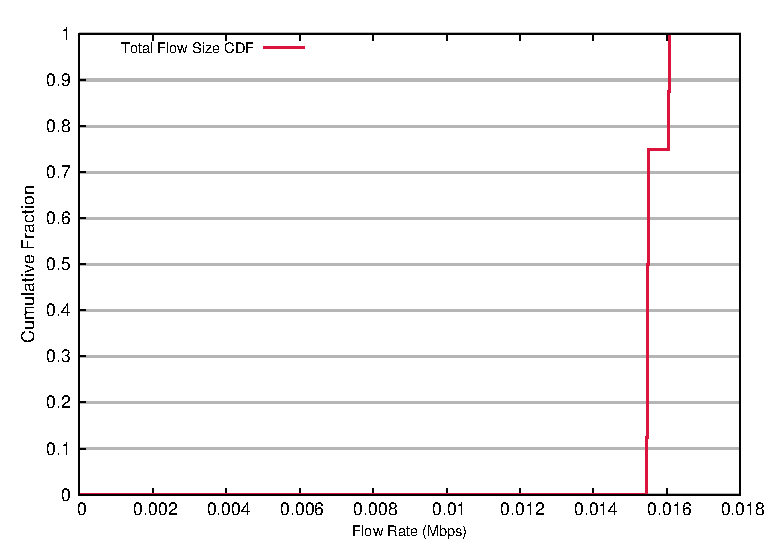
\includegraphics[width=.55\textwidth]{figures/4read/24_28_flow_size.eps} &
%	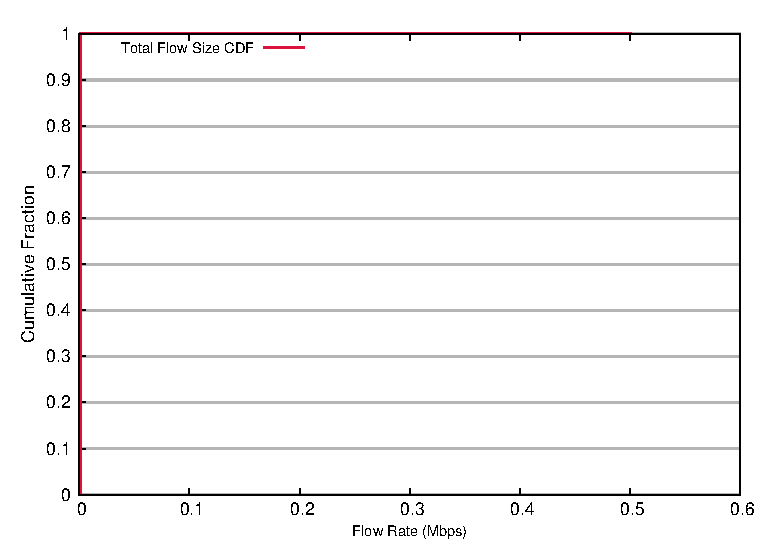
\includegraphics[width=.55\textwidth]{figures/4read/8_12_flow_size.eps}  \\
%	\multicolumn{2}{c}{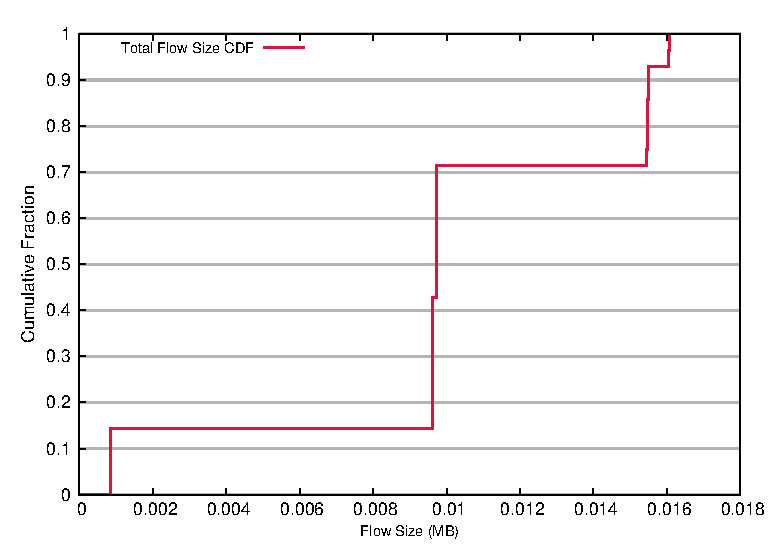
\includegraphics[width=.73\textwidth]{figures/4read/flow_size.eps}}
%    \end{tabular}
%\caption{Read Flow Size Distribution}
%\end{figure*}
%\end{comment}

\begin{figure*}[!ht]
\label{fig:read_size}
\centering
  \begin{subfigure}[b]{.45\linewidth}
   \centering
	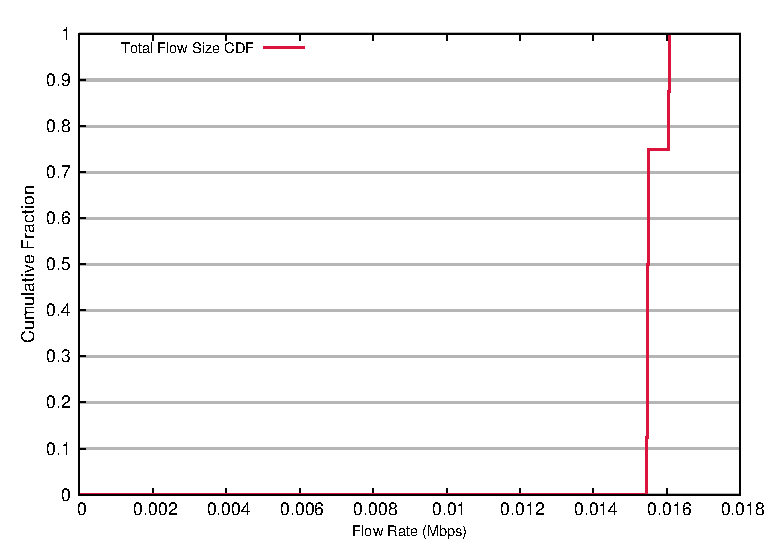
\includegraphics[width=.99\textwidth]{figures/4read/24_28_flow_size.eps} 
	\caption{RPC between Client and DataNodes}\label{fig:read_size:rpc}
   \end{subfigure}%
  \begin{subfigure}[b]{.45\linewidth}
   \centering
	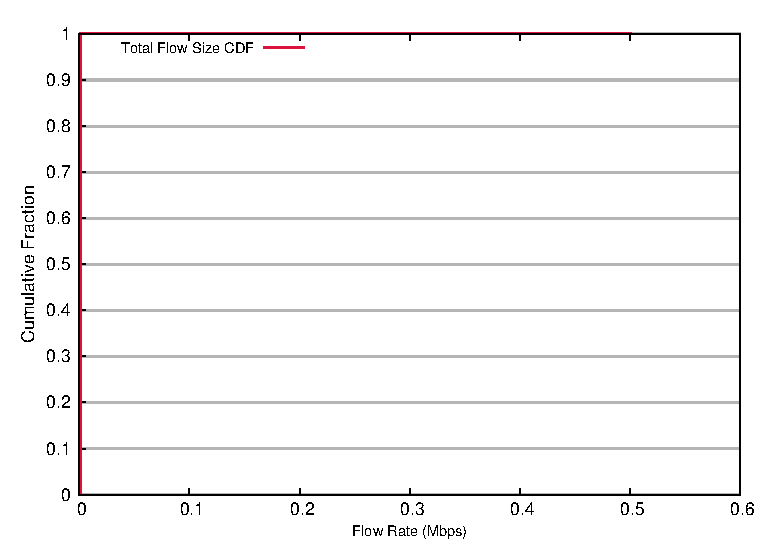
\includegraphics[width=.99\textwidth]{figures/4read/8_12_flow_size.eps} 
	\caption{Should have read data transfer here}\label{fig:read_size:fixme}
   \end{subfigure} \\%
  \begin{subfigure}[b]{.75\linewidth}
   \centering
	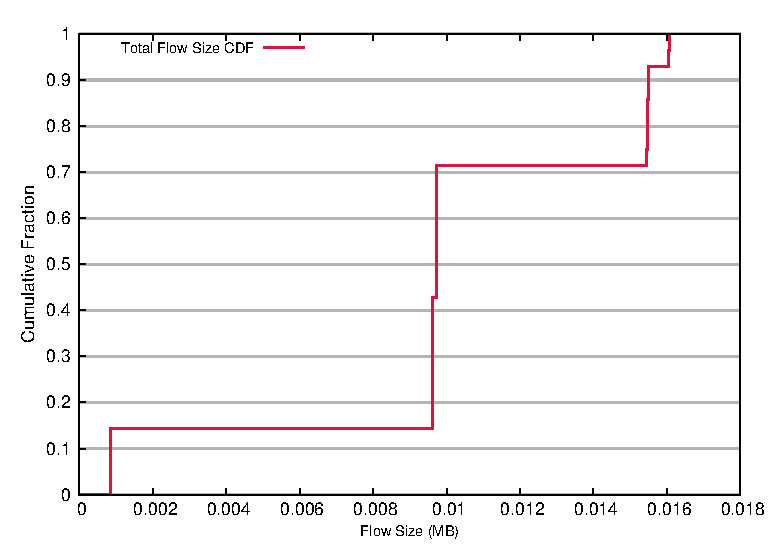
\includegraphics[width=.99\textwidth]{figures/4read/flow_size.eps}
	\caption{All Traffic}\label{fig:read_size:all}
   \end{subfigure}%
\caption{Read Flow Size Distribution}
\end{figure*}

FXIME: read workload doesn't make sense here, needs to fix it.


\begin{figure*}[!ht]
\label{fig:write_size}
\centering
  \begin{subfigure}[b]{.45\linewidth}
   \centering
	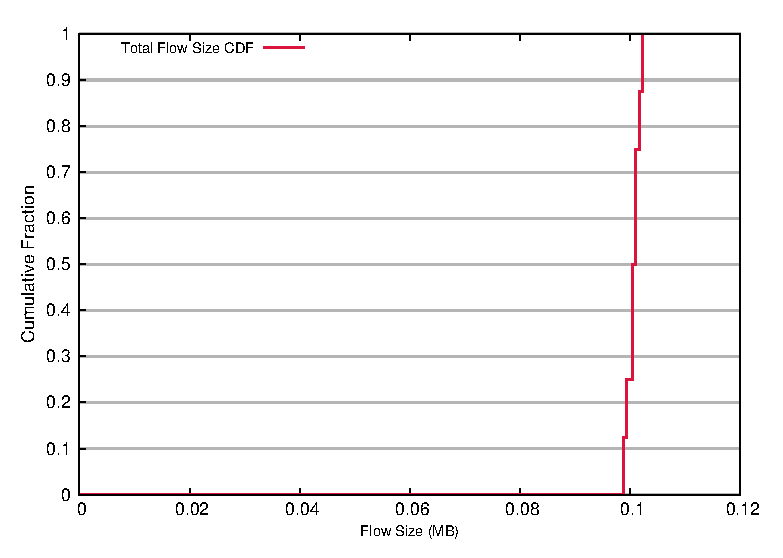
\includegraphics[width=.99\textwidth]{figures/6writes/24_28_type_flow_size.eps} 
	\caption{DataNodes RPC with NameNode}\label{fig:write_size:dn_rpc}
   \end{subfigure}%
  \begin{subfigure}[b]{.45\linewidth}
   \centering
	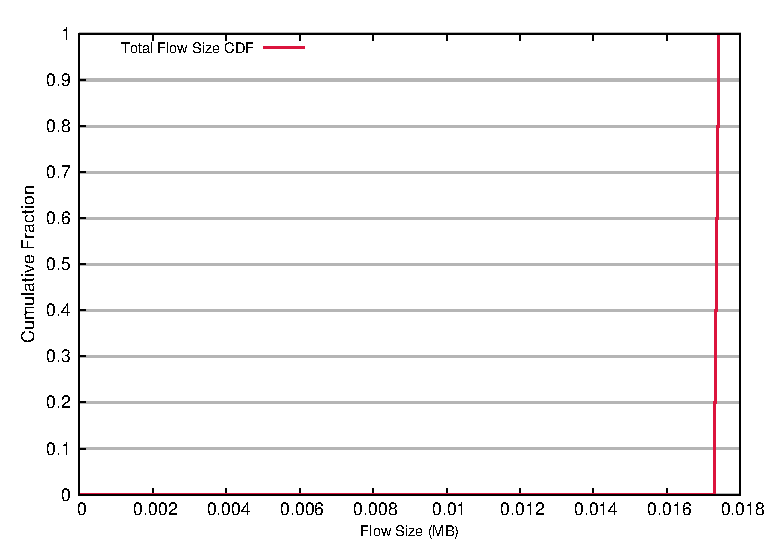
\includegraphics[width=.99\textwidth]{figures/6writes/24_28_20_16_type_flow_size.eps} 
	\caption{Client and DataNodes RPC with NameNode}\label{fig:write_size:dc_rpc}
   \end{subfigure} \\%
  \begin{subfigure}[b]{.45\linewidth}
   \centering
	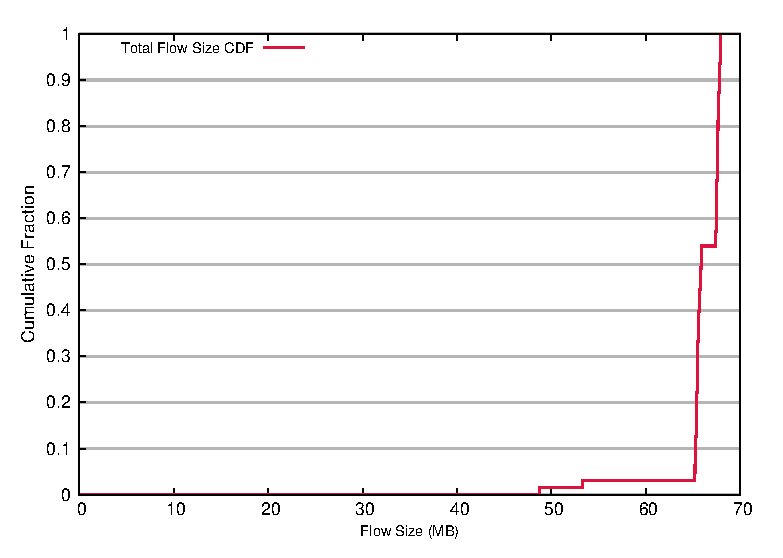
\includegraphics[width=.99\textwidth]{figures/6writes/36_44_type_flow_size.eps} 
	\caption{Pipelined Writes between DataNodes}\label{fig:write_size:pipe_write}
   \end{subfigure} %
  \begin{subfigure}[b]{.45\linewidth}
   \centering
	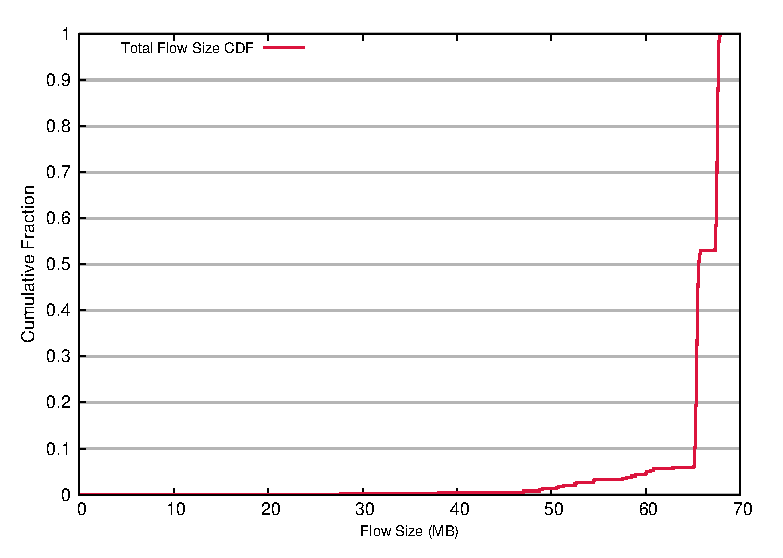
\includegraphics[width=.99\textwidth]{figures/6writes/32_36_type_flow_size.eps} 
	\caption{Client Data Transfer to DataNodes}\label{fig:write_size:client_write}
   \end{subfigure} \\%
  \begin{subfigure}[b]{.75\linewidth}
   \centering
	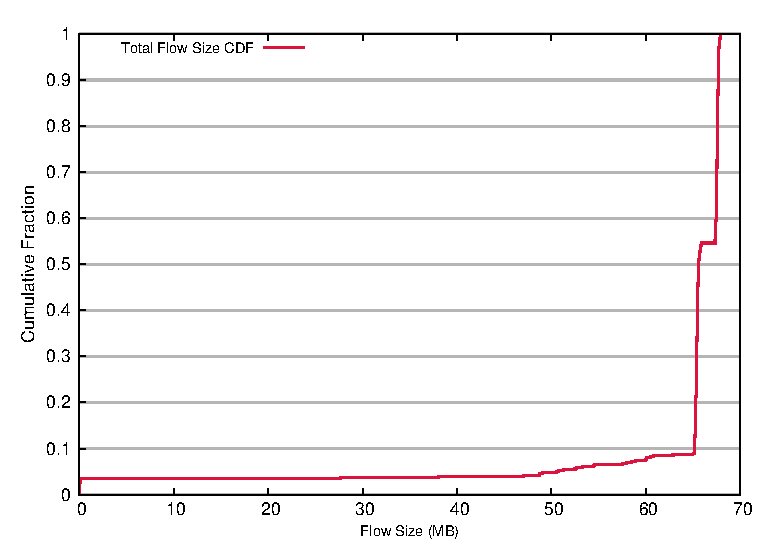
\includegraphics[width=.99\textwidth]{figures/6writes/flow_size.eps}
	\caption{All Traffic}\label{fig:write_size:all}
   \end{subfigure}%
\caption{Write Flow Size Distribution}
\end{figure*}


The flow size distribution of the write workload shown in figure \ref{fig:write_size} revealed some information about HDFS's internal operation. We can see that there are twon kinds of flows, RPC flows, which typically has very small data transferred; and data transfer flows, including the pipelined data transfer between data nodes and the data client writes to the datanodes, which is around 65 MB. This is in compliance with the fact that HDFS has separate flows for RPC calls/responses and data transfers; and data transfer is done in the unit of blocks, which is 64 MB in our configuration. We could also see that less than 5\% of the flows are used for RPC calls to transfer control information, while the majority of the flows are used for data transfer, which is as expected. 

\begin{figure*}[!ht]
\label{fig:replica_size}
\centering
  \begin{subfigure}[b]{.45\linewidth}
   \centering
	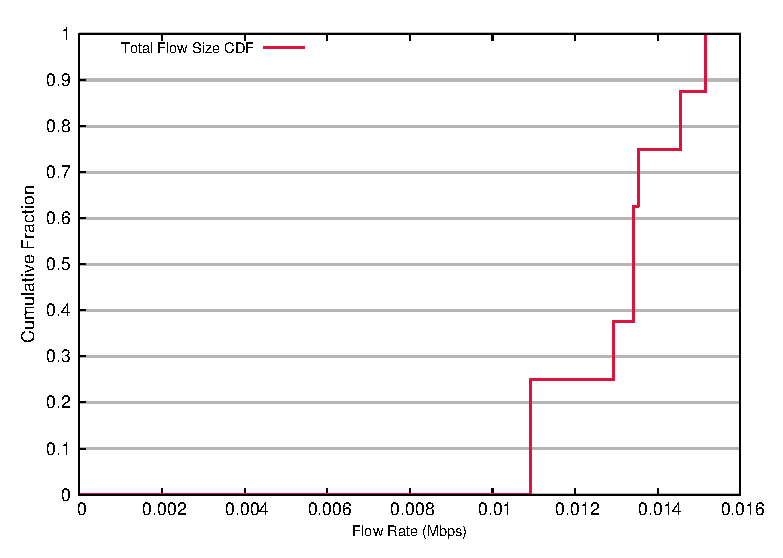
\includegraphics[width=.99\textwidth]{figures/replica_change/24_28_flow_size.eps} 
	\caption{DataNodes RPC with NameNode}\label{fig:replica_size:rpc}
   \end{subfigure}%
  \begin{subfigure}[b]{.45\linewidth}
   \centering
	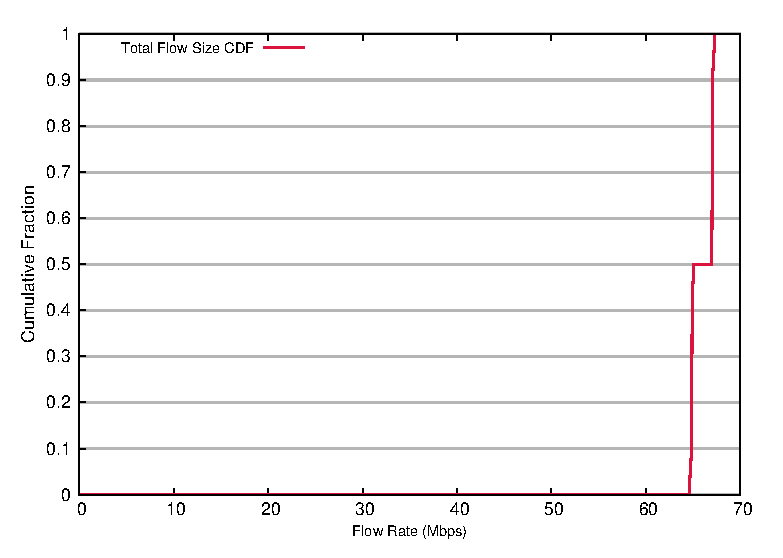
\includegraphics[width=.99\textwidth]{figures/replica_change/36_32_flow_size.eps} 
	\caption{Pipelined Writes between DataNodes}\label{fig:replica_size:pipe_write}
   \end{subfigure} \\%
  \begin{subfigure}[b]{.75\linewidth}
   \centering
	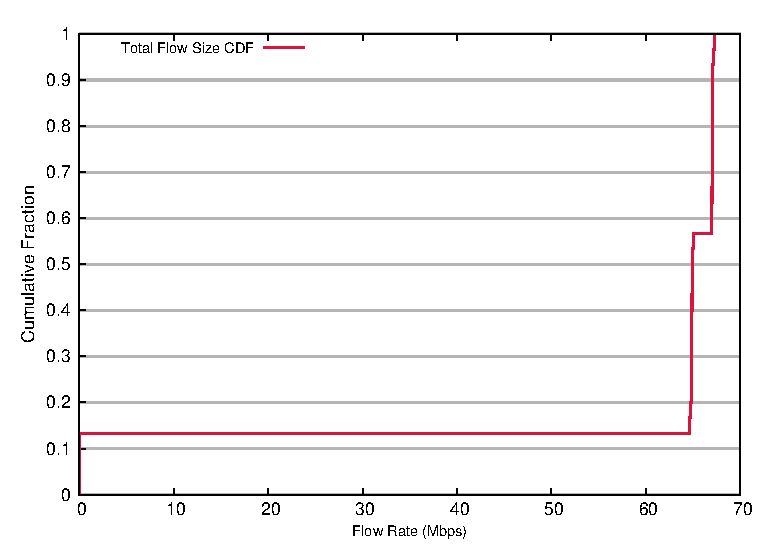
\includegraphics[width=.99\textwidth]{figures/replica_change/flow_size.eps}
	\caption{All Traffic}\label{fig:read_size:all}
   \end{subfigure}%
\caption{Replciation Level Change Flow Size Distribution}
\end{figure*}

The flow size distribution of the replication level change workload in figure \ref{fig:replica_size} exihibed the same characteristics, except for that we have less data transfers and relatively more control messages. 


\subsection{\bf Flow Duration Analysis}
The flow duration distributions for each kind of workloads are shown in figure \ref{fig:read_duration}, \ref{fig:write_duration} and \ref{fig:replica_duration}.

\begin{figure*}[!htpb]
\centering
  \begin{subfigure}[b]{.45\linewidth}
   \centering
	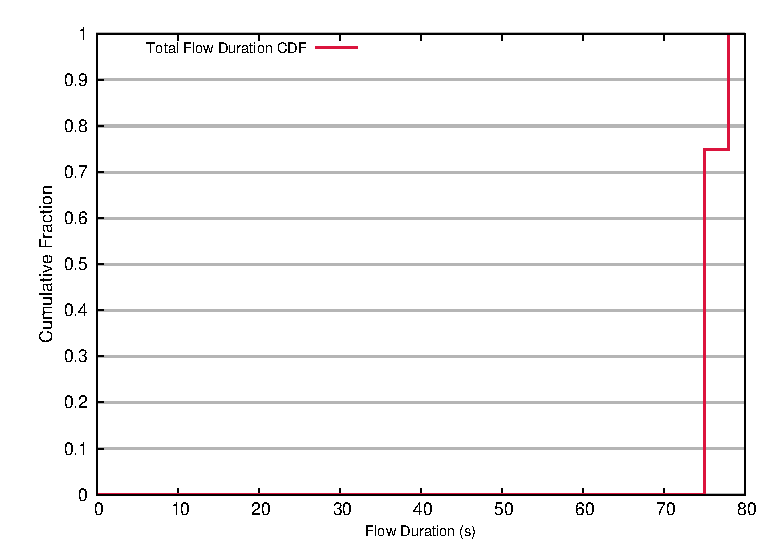
\includegraphics[width=.99\textwidth]{figures/4read/24_28_type_duration.eps} 
	\caption{RPC between Client and DataNodes}\label{fig:read_duration:rpc}
   \end{subfigure}%
  \begin{subfigure}[b]{.45\linewidth}
   \centering
	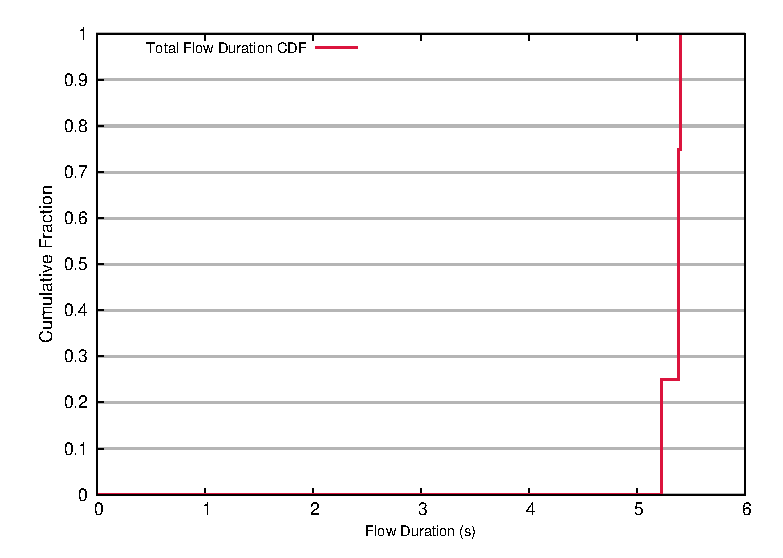
\includegraphics[width=.99\textwidth]{figures/4read/24_28_20_16_type_duration.eps} 
	\caption{Client and DataNodes RPC with NameNode}\label{fig:read_duration:nn_rpc}
   \end{subfigure} \\%
  \begin{subfigure}[b]{.55\linewidth}
   \centering
	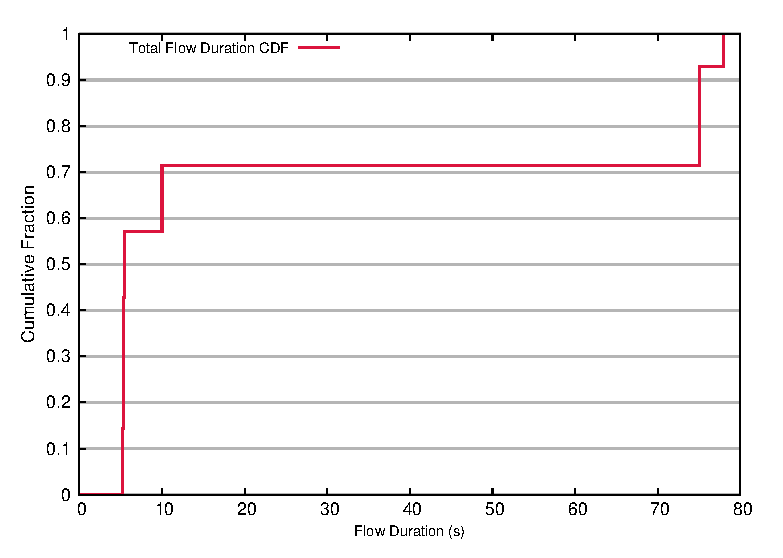
\includegraphics[width=.99\textwidth]{figures/4read/flow_duration.eps}
	\caption{All Traffic}\label{fig:read_duration:all}
   \end{subfigure}%
\caption{Read Flow Duration Distribution}
\label{fig:read_duration}
\end{figure*}

Again, we could see in figure \ref{fig:read_duration} that for the read workloads, almost all the flows are long lived RPC flows.

\begin{figure*}[!htbp]
\centering
  \begin{subfigure}[b]{.45\linewidth}
   \centering
	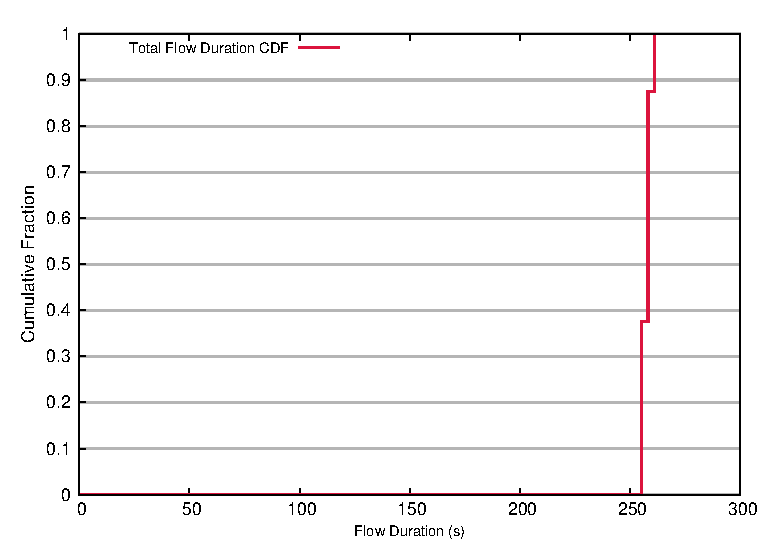
\includegraphics[width=.99\textwidth]{figures/6writes/24_28_type_flow_duration.eps} 
	\caption{DataNodes RPC with NameNode}\label{fig:write_duration:dn_rpc}
   \end{subfigure}%
  \begin{subfigure}[b]{.45\linewidth}
   \centering
	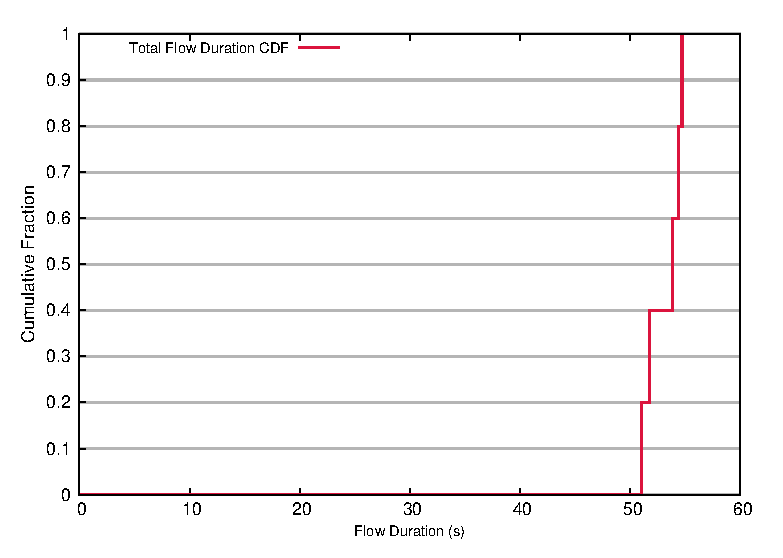
\includegraphics[width=.99\textwidth]{figures/6writes/24_28_20_16_type_flow_duration.eps} 
	\caption{Client and DataNodes RPC with NameNode}\label{fig:write_duration:dc_rpc}
   \end{subfigure} \\%
  \begin{subfigure}[b]{.45\linewidth}
   \centering
	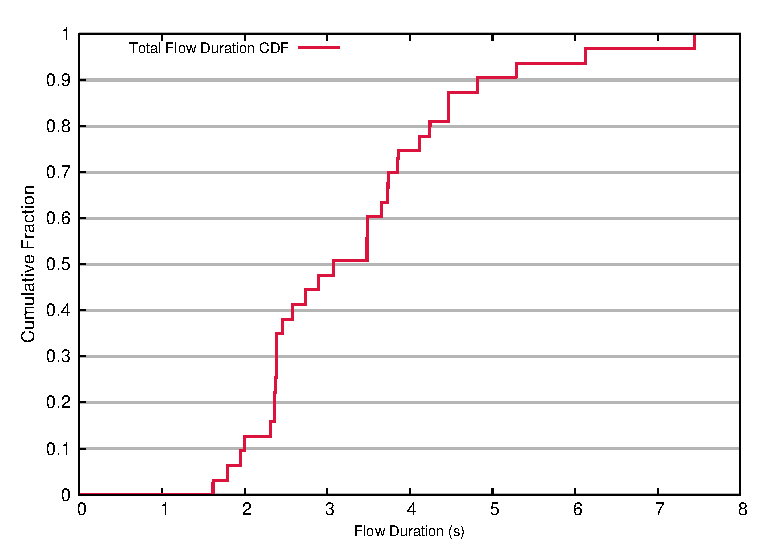
\includegraphics[width=.99\textwidth]{figures/6writes/36_44_type_flow_duration.eps} 
	\caption{Pipelined Writes between DataNodes}\label{fig:write_duration:pipe_write}
   \end{subfigure} %
  \begin{subfigure}[b]{.45\linewidth}
   \centering
	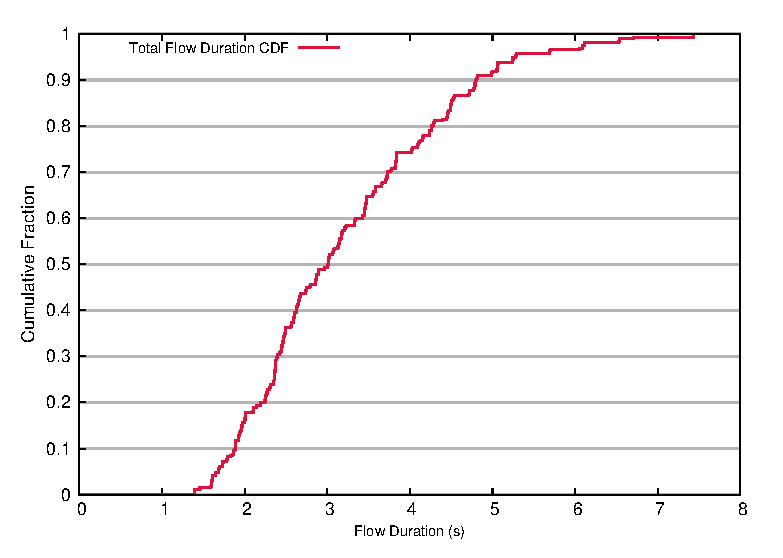
\includegraphics[width=.99\textwidth]{figures/6writes/32_36_type_flow_duration.eps} 
	\caption{Client Data Transfer to DataNodes}\label{fig:write_duration:client_write}
   \end{subfigure} \\%
  \begin{subfigure}[b]{.45\linewidth}
   \centering
	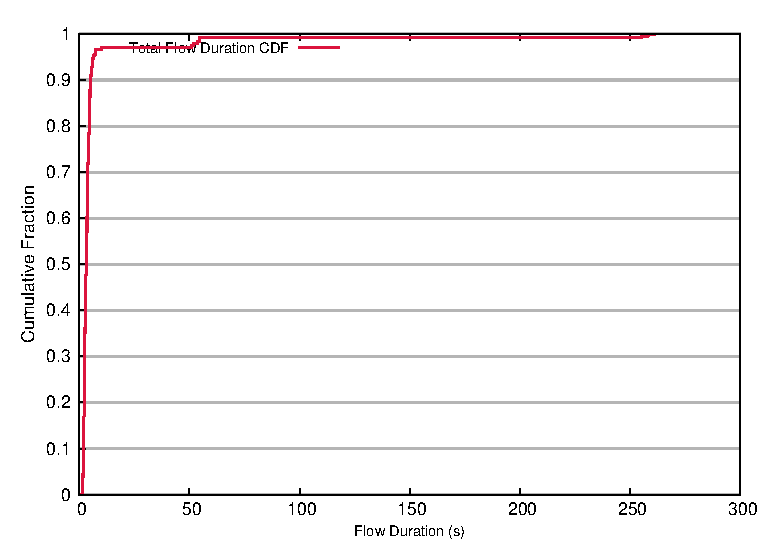
\includegraphics[width=.99\textwidth]{figures/6writes/flow_duration.eps}
	\caption{All Traffic}\label{fig:write_duration:all}
   \end{subfigure}%
  \begin{subfigure}[b]{.45\linewidth}
   \centering
	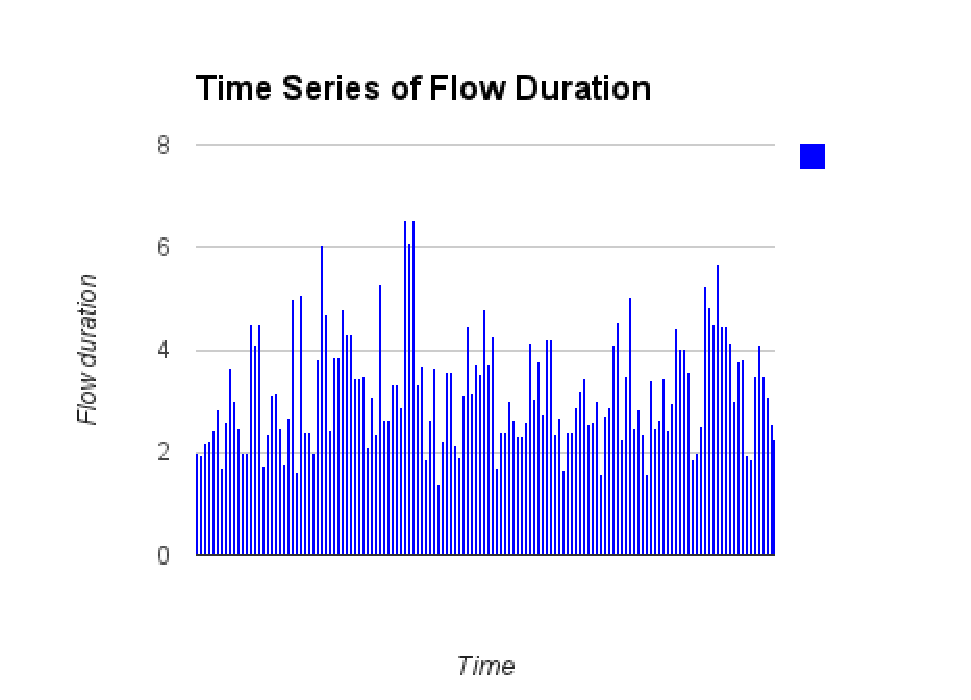
\includegraphics[width=.99\textwidth]{figures/6writes/flow_duration_time_series.eps}
	\caption{Time Series of All Traffic}\label{fig:write:time_series}
   \end{subfigure}%
\caption{Write Flow Duration Distribution}
\label{fig:write_duration}
\end{figure*}

For the write workload, we can again see the radical differences between RPC calls/responds flows, which are long lived and shared among multiple RPC calls; and data transfer flows, which transfers one block of file data in HDFS in its lifetime. However, we have noticed that the data transfer flows' duration spans a wide range, from less than 2 seconds to more than seven seconds, even though all of them transfer the same amount of data. In order to determine whether this is caused by network congestion or any hotspots within the network, we looked the flow duration on each link of the network, and found that this distribution is not dependent on the network location. Actually flows between any two nodes in our network exhibit the similar duration distribution (results omitted in the interest of space). The time series of the flow duration is also shown in figure \ref{fig:write:time_series}, and we could see periodic spike in the flow duration. We think it could be related to the network condition, but no further information is available to investigate the cause of it.

\begin{figure*}[!htbp]
\centering
  \begin{subfigure}[b]{.45\linewidth}
   \centering
	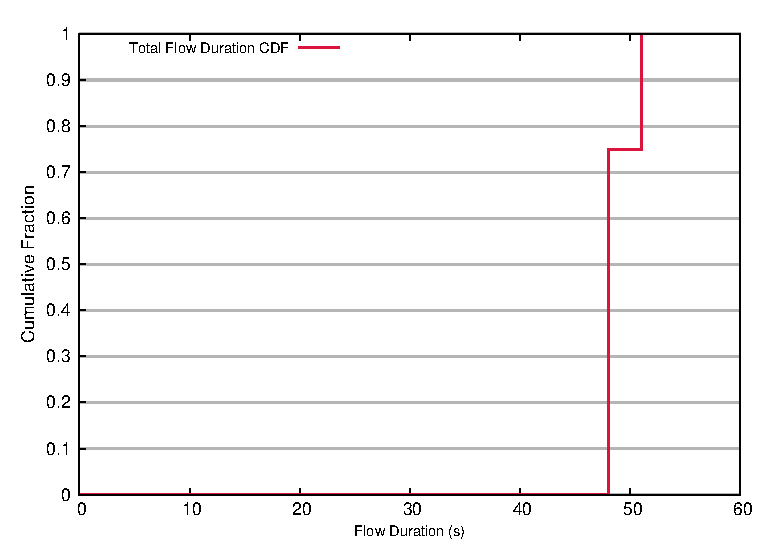
\includegraphics[width=.99\textwidth]{figures/replica_change/24_28_flow_duration.eps} 
	\caption{DataNodes RPC with NameNode}\label{fig:replica_duration:rpc}
   \end{subfigure}%
  \begin{subfigure}[b]{.45\linewidth}
   \centering
	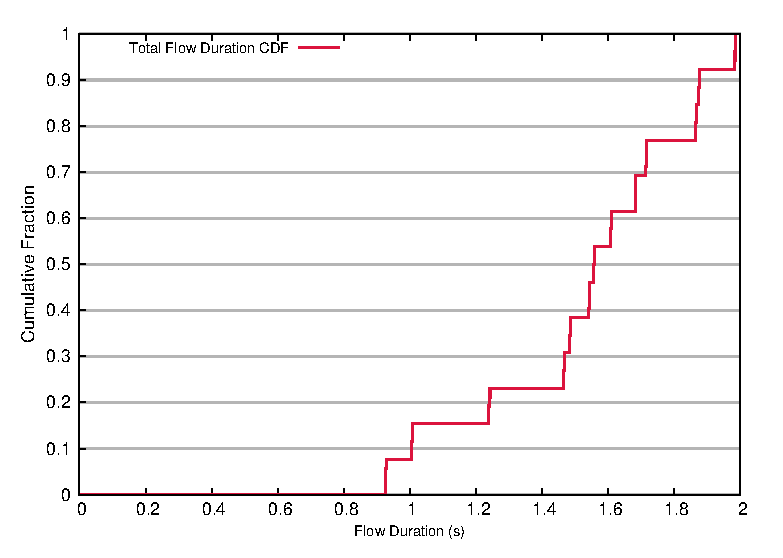
\includegraphics[width=.99\textwidth]{figures/replica_change/36_32_flow_duration.eps} 
	\caption{Pipelined Writes between DataNodes}\label{fig:replica_duration:pipe_write}
   \end{subfigure} \\%
  \begin{subfigure}[b]{.55\linewidth}
   \centering
	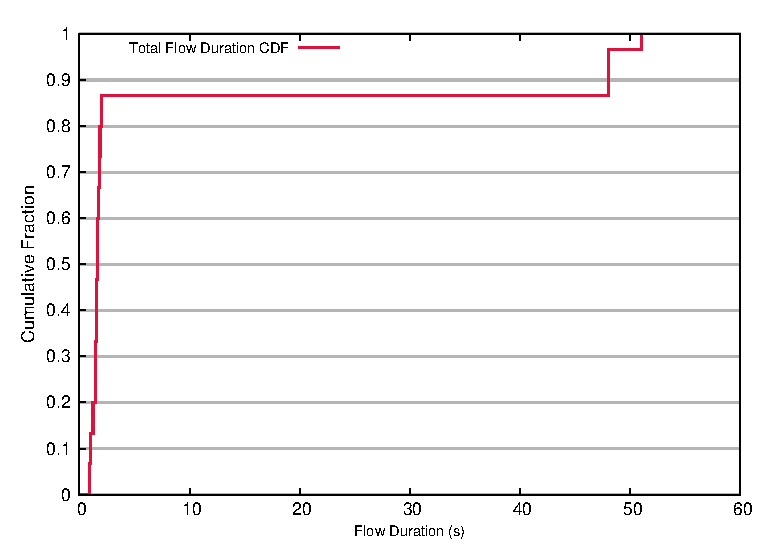
\includegraphics[width=.99\textwidth]{figures/replica_change/flow_duration.eps}
	\caption{All Traffic}\label{fig:read_duration:all}
   \end{subfigure}%
\caption{Replciation Level Change Flow Duration Distribution}
\label{fig:replica_duration}
\end{figure*}

The flow duration distribution of the replication level change workload in figure \ref{fig:replica_duration} exhibit the same characteristics, except for that there is fewer data transfered, thus flows are generally shorter. 



\section{Related Work}
Recent years data centers have seen great changes. Multi-tenant public cloud such as Amazon EC2 and ever larger data centers have been popular. A huge amount of data-intensive and web serving applications have become dominant workloads in the data center. The storage and network also evolve to better serve these applications. New data center network architectures also emerge, e.g., c-through~\cite{c-through} proposes a hybrid packet and circuit switched network architecture to supply high bandwidth to applications. Helios~\cite{helios} is a hybrid electrical/optical switch architecture to ease the deployment of modular data centers. Flyaways~\cite{flyaways} proposes to use the wireless links to selectively add capacity where needed. At the same time, many cloud systems adopt key-value stores or NoSQL systems such as BigTable, HBase, Cassandra and Voldemort, and different components in these distributed storage systems rely on the network to communicate with each other.

Some research works already reveal that the network architecture and how network behaves have great impact on storage performance. Flat Datacenter Storage (FDS)~\cite{flat-datacenter-storage} is a recent work which exploits full bisection bandwidth networks to obviate the need of data locality and enables to expose all of a cluster's disk bandwidth to applications. Incast~\cite{incast} problem could happen when a client synchronously reads fragments of a data block from multiple data sources.

Yet little work is done about the interaction between storage and network. For example, Pisces~\cite{pisces} provides performance isolation and fairness between tenants, but it assumes network is well provisioned. On the other hand, FairCloud~\cite{faircloud} proposes network allocation policies to better achieve fairness in cloud environment but does not touch storage. Moreover, network optimizations for data-intensive applications such as Orchestra~\cite{orchestra} often assume all data can be accommodated in memory and therefore ignore the storage I/O cost. But ~\cite{c-through} points out that these applications can still be bottlenecked by intensive disk I/O operations.

Conventional network measurement such as~\cite{wild} usually concerns about the network traffic as a whole rather than pays particular attention to storage system traffics.


\nocite{*}
%\begin{small}
\bibliographystyle{abbrv}
\bibliography{refs}
%\end{small}

\end{document}
